\let\negmedspace\undefined
\let\negthickspace\undefined
\documentclass[journal]{IEEEtran}
\usepackage[a5paper, margin=10mm, onecolumn]{geometry}
%\usepackage{lmodern} % Ensure lmodern is loaded for pdflatex
\usepackage{tfrupee} % Include tfrupee package

\setlength{\headheight}{1cm} % Set the height of the header box
\setlength{\headsep}{0mm}     % Set the distance between the header box and the top of the text

\usepackage{gvv-book}
\usepackage{gvv}
\usepackage{cite}
\usepackage{amsmath,amssymb,amsfonts,amsthm}
\usepackage{algorithmic}
\usepackage{graphicx}
\usepackage{textcomp}
\usepackage{xcolor}
\usepackage{txfonts}
\usepackage{listings}
\usepackage{enumitem}
\usepackage{mathtools}
\usepackage{gensymb}
\usepackage{comment}
\usepackage[breaklinks=true]{hyperref}
\usepackage{tkz-euclide} 
\usepackage{listings}
% \usepackage{gvv}                                        
\def\inputGnumericTable{}                                 
\usepackage[latin1]{inputenc}                                
\usepackage{color}                                            
\usepackage{array}                                            
\usepackage{longtable}                                       
\usepackage{calc}                                             
\usepackage{multirow}                                         
\usepackage{hhline}                                           
\usepackage{ifthen}                                           
\usepackage{lscape}

\renewcommand{\thefigure}{\theenumi}
\renewcommand{\thetable}{\theenumi}
\setlength{\intextsep}{10pt} % Space between text and floats


\numberwithin{equation}{enumi}
\numberwithin{figure}{enumi}
\renewcommand{\thetable}{\theenumi}

% Marks the beginning of the document
\begin{document}
\bibliographystyle{IEEEtran}

\title{10.4.4.2.1}
\author{EE24BTECH11049 - Patnam Shariq Faraz Muhammed}

% \maketitle
% \newpage
% \bigskip
{\let\newpage\relax\maketitle}

\textbf{Question:}\\

Find the values of k for which the quadratic equation $2x^2 + kx + 5 = 0$. So they've two equal roots.\\

\textbf{Solution:}\\

Given Equation:
\begin{align}
    2x^2 + kx + 5 = 0
\end{align}

\textbf{Numerical Solution:}
\begin{itemize}
    \item If the roots are equal then the value of Discriminant is to $0$
        \begin{align}
            b^2 - 4ac &= 0\\
            k^2 - 4 \times 2 \times 5 &= 0\\\
            k &= \pm 2\sqrt{10}
        \end{align}
        We get two equations since there are two values for k.
        \begin{align}
            2x^2 + 2\sqrt{10}x + 5 &= 0 \label{Quad1}\\
            2x^2 - 2\sqrt{10}x + 5 &= 0 \label{Quad2}
        \end{align}
    \item They've a single root that is $\frac{-b}{2a}$.\\
        \begin{itemize}
            \item root of \eqref{Quad1} = $-\sqrt{\frac{5}{2}}$\\
            \item root of \eqref{Quad2} = $+\sqrt{\frac{5}{2}}$\\
        \end{itemize}
\end{itemize}

\newpage
\textbf{Computational Solutions:}
\begin{enumerate}
    \item \textbf{Fixed Point iteration}
    \begin{itemize}
        \item The fixed point iteration method in numerical analysis is used to find an approximate solution to algebraic and transcendental equations.
        \item \textbf{How it works?}
        \begin{itemize}
            \item Rewrite into $X = g\brak{x}$
            \item Idea the root is $r = g\brak{r}$, $r$ = fixed Point
            \item initial guess $= x_0$, compute $g\brak{x_0}$
            \item Hopefully $x_1 = g\brak{x_0}$ is closer to $r$ \brak{\text{Occurs when it's convergence}}
            \item Do iteration until stop criteria
            \begin{align}
                x_{n + 1} = g\brak{x_n}
            \end{align}
            \item end
        \end{itemize}
        \item \textbf{Stop Criteria:}
        \begin{align}
            \abs{x_{n + 1} - x_n} \leq tolerence\\
            \abs{g\brak{x_n} - x_n} \leq tolerence
        \end{align}
        \item This algorithm succeeds with proper choice of $g\brak{x}$ and must be convergent 
        \item \textbf{Error Analysis:}
        \begin{itemize}
            \item Let $r$ be the root, that is, $r = g\brak{r}$ 
            \item Iteration: 
            \begin{align}
                x_{n + 1} = g\brak{x_n}
            \end{align}
            \item Error $e$:
            \begin{align}
                e_n &= \abs{x_n - r}\\
                e_{n + 1} &= \abs{x_{n + 1} - r}\\
                &= \abs{g\brak{x_n} - g\brak{r}}\\
                &= \abs{g^{\prime}\brak{c}} \abs{x_n - r} \text{ where, } x_n < c < r\\
                &= \abs{g^{\prime}\brak{c}} e_n
            \end{align}
            \item Observation: 
            \begin{itemize}
                \item If $\abs{g^{\prime}\brak{c}} < 1 \implies e_{n + 1} < e_n $: convergence.
                \item If $\abs{g^{\prime}\brak{c}} > 1 \implies e_{n + 1} > e_n $: Divergence.
            \end{itemize}
        \end{itemize}
        \item \textbf{Convergence Condition:} 
        There exist an interval $ I = \sbrak{r - c, r + c}$ for some $c > 0$ such that $\abs{g^{\prime}\brak{x}} < 1$ on $I$ and $x_0 \in I$
        \begin{table}[!ht]
            \centering
            \begin{tabular}{|c|c|}
    \hline
    \textbf{Variable} & \textbf{Description}\\
    \hline
    $P_0$ & initial principal amount\\
    \hline
    $r$ & rate of increase per year\\
    \hline
    $t$ & time in years\\
    \hline 
    $C \& C_1$ & arbitrary constants\\
    \hline
    $P$ & principal at any time $t$\\
    \hline
\end{tabular}

            \caption{Fixed point iteration}
            \label{fpi}
        \end{table}
        \item For the given Question there are 2 choices for each Quadratic
        \item For all $g\brak{x}$, fixed point algo diverges.
        \item Initial guess\\
        Quad1: x0 = -5, x1 = -3, x2 = 0, x3 = 2\\
        Quad2: x0 = -2, x1 = 0, x2 = 3, x3 = 5
        \item \textbf{Program Output:}
        \begin{multicols}{2}
        Quad1:\\
        $g_1$\\
        Guess 1 failed for root\\
        Guess 2 failed for root\\
        Failed to detect root.\\
        Guess 1 failed for root\\
        Guess 2 failed for root\\
        Failed to detect root.\\
        Fixed-point iteration failed to converge.\\
        $g_3$\\
        Guess 1 failed for root\\
        Guess 2 failed for root\\
        Failed to detect root.\\
        Guess 1 failed for root\\
        Guess 2 failed for root\\
        Failed to detect root.\\
        Fixed-point iteration failed to converge.\\
        \columnbreak
        \\
        Quad2:\\
        $g_2$\\
        Guess 1 failed for root\\
        Guess 2 failed for root\\
        Failed to detect root.\\
        Guess 1 failed for root\\
        Guess 2 failed for root\\
        Failed to detect root.\\
        Fixed-point iteration failed to converge.\\
        $g_4$\\
        Guess 1 failed for root\\
        Guess 2 failed for root\\
        Failed to detect root.\\
        Guess 1 failed for root\\
        Guess 2 failed for root\\
        Failed to detect root.\\
        Fixed-point iteration failed to converge.\\
        \end{multicols}

    \end{itemize}
    \item \textbf{Newton's Method}
    \begin{itemize}
        \item Newton's Method is an iterative numerical technique used to approximate the roots of a real-valued function. It's particularly effective when you have a good initial guess for the root.
        \item Newton's Method uses the idea of approximating a function by its tangent line at a given point:
        \begin{align}
            x_{n + 1} = x_n - \frac{f\brak{x_n}}{f^{\prime}\brak{x_n}}
        \end{align}
        \item It is iterated until convergence.
        \item We can view newton's method as "optimal" fixed point because $g^{\prime}\brak{r}$ = 0
        \begin{align}
            x_{n + 1} &= g\brak{x_n} = x_n - \frac{f\brak{x_n}}{f^{\prime}\brak{x_n}}\\
            g^{\prime}\brak{x} &= \frac{f\brak{x}f^{\prime\prime}\brak{x}}{\brak{f^{\prime}\brak{x}}^2}\\
            f\brak{r} &= 0 \implies g^{\prime}\brak{r} = 0
        \end{align}
        \item \textbf{Error Analysis:}\\
        \begin{itemize}
            \item Error $e_k$ = $\abs{x_n - r}$\
            From Taylor's expansion, Final result
            \begin{align}
                e_{n + 1} \leq \frac{1}{2} max{\abs{g^{\prime\prime}\brak{c}}}e_n^2
            \end{align}
            \item It exhibits quadratic convergence near the root, provided the initial guess is close enough, the function is sufficiently smooth, and the derivative at the root is not zero. 
            \item This means the error roughly squares with each iteration, making Newton's method much faster once it's near the solution.
        \end{itemize}
    \item \textbf{Result:}
    \begin{itemize}
        \item By taking the initial guesses -3 and 0 (assuming it has two roots)for the first quadratic \eqref{Quad1} we get the result in 24 iterations. 
        \begin{align}
            x = -1.5811389
        \end{align}
        \item By taking the initial guesses 3 and 0 (assuming it has two roots)for the second quadratic \eqref{Quad2} we get the result in 24 iterations. 
        \begin{align}
            x = 1.5811389
        \end{align}
    \end{itemize}
    \end{itemize}
    \begin{multicols}{2}	
	\begin{figure}[H]
   \centering
   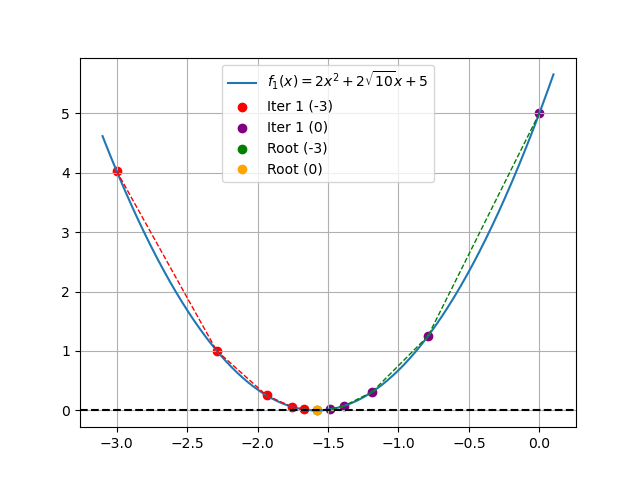
\includegraphics[width=1\columnwidth]{figs/fig1.png}
   \caption{Root of the function1}
\end{figure}
\begin{figure}[H]
   \centering
   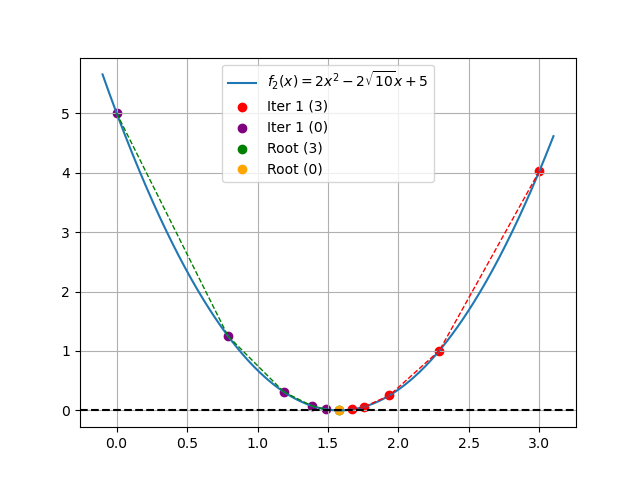
\includegraphics[width=1\columnwidth]{figs/fig2.png}
   \caption{Root of the function2}
\end{figure}
    \end{multicols}
    %figs
    \item \textbf{Secant Method}
    \begin{itemize}
        \item It's a Hybrid idea(variant) of newton's and more robust.
        \item We need to obtain a good initial Guess $x_0$ And apply newton's to it.
        \item In this method we can avoid computing $f^{\prime}\brak{x}$
        \item In newton's we use an tangent line, here we use secant for approximation
        \item secant's iteration:
        \begin{align}
            x_{n + 1} = x_n - f\brak{x_n}\frac{x_n - x_{n - 1}}{f\brak{x_n} - f\brak{x_{n - 1}}}
        \end{align}
        \item \textbf{Advantages:}
        \begin{itemize}
            \item No computation of $f^{\prime}\brak{x}$
            \item One function per iteration is calculated
            \item Very rapid convergence
        \end{itemize}
        \item \textbf{Error}
        \begin{align}
            e_{k + 1} \leq M. e_k^{\alpha} \text{ Where } \alpha = \frac{1}{2}\brak{1 + \sqrt{5}}
        \end{align}
        It is super linear convergence since $1 < \alpha < 2$\\
        \item \textbf{Failure} 
        \begin{itemize}
            \item For the both the quadratic equations the secant's algo fails to find the root. Output: Difference of the functions is too small.
            \item This shows us that both the Quadratics have roots as their minimum values.
            \item The secant method fails at minima or maxima of that function
            \begin{itemize}
                \item The slope between two points is almost zero.
                \item The secant line becomes nearly horizontal, and the intersection with the x-axis is poorly defined.
            \end{itemize}
        \end{itemize}
    \end{itemize}
    \item \textbf{Matrix Method}\\
    If we consider the polynomial equation as the characteristic equation of a matrix, then by finding the eigen-values of that matrix, we can find the roots of the equation.\\
    The matrix whose eigen-values are the roots of polynomial equation is called the companion matrix of the said equation.
     If the given polynomial is,
     \begin{align}
     	P(x) = c_0 + c_1\,x + c_2\,x^2 + \dots + c_{n-1}\,x^{n-1} + c_nx^n
     \end{align}
     The companion matrix of this polynomial can be written as
     \begin{align}
          c = \myvec{0 & 0 & \dots & 0 & -\frac{c_0}{c_n}\\1 & 0 & \dots & 0 & -\frac{c_1}{c_n}\\0 & 1 & \dots & 0 & -\frac{c_2}{c_n}\\\vdots & \vdots & \vdots & \vdots &\vdots \\0 & 0 & \dots & 1 & -\frac{c_{n - 1}}{c_n}} \label{comp}
     \end{align}
    \textbf{Power Iteration}
    \begin{itemize}
        \item The Power iteration finds the largest eigen value $\lambda_{max}$ of a companion matrix 
        \item now divide the polynomial with $x - \lambda_{max}$ by performing synthetic division. This results in a new polynomial of degree one less.
        \item Repeat this process the degree becomes one.
    \end{itemize}

    The power Iteration follows the following steps iteratively:
    \begin{align}
        \Tilde{\vec{v_n}} &= C\vec{v_{n - 1}}\\
        \vec{v_n} &= \frac{\Tilde{\vec{v_n}}}{\norm{\Tilde{\vec{v_n}}}}
    \end{align}

     This iteration stops when
     \begin{align}
         \abs{\lambda_{max}^{\brak{n}} - \lambda_{max}^{\brak{n - 1}}} < \epsilon
     \end{align}
     After $\epsilon$ is tolerance, and 
     \begin{align}
         \lambda_n = \frac{\vec{x_n}^{\top} C \vec{x_n}}{\vec{x_n}^{\top}\vec{x_n}}
     \end{align}
     Once $\lambda_{\text{max}}$ is found, synthetic division is performed to reduce the polynomial:
     \begin{align}
     	P(x) &= P(x) \div (x - \lambda_{\text{max}}), \\
     	P(x) &= c_{1,0} + c_{1,1}x + c_{1,2}x^{2} + \cdots + c_{1,(n-1)}x^{n-1}.
     \end{align}
     Now, the new companion matrix will be evaluated.  
     
     This process is repeated iteratively until the polynomial is reduced to a degree-1 equation:
     \begin{align}
     	P_1(x) = c_{n-1,0} + c_{n-1,1}x.
     \end{align}
     Thus, the effective update equation would be:
     \begin{align}
     	P_{n-1}(x) &= P_{n}(x) \div (x - \lambda_{n}),
     \end{align}
     \item \textbf{Time complexity}
     \begin{itemize}
        \item The construction of the companion matrix: $O(n^2)$.
        \item The power iteration process: $O(k \cdot n^2)$, where $k$ is the number of iterations required for convergence.
        \item Synthetic division: $O(n)$.
     \end{itemize}     
\end{enumerate}
\end{document}
